Because the tower height varied in this study, it was necessary to calculate the tower mass and perform structural analyses.
%We modeled the tower as a tapered steel cylinder. As shown in Fig. \ref{tower_def}, the tower diameter and shell thickness were parameterized at the bottom, midpoint, and top of the tower, and were linearly interpolated in between.
The structural analysis was used to constrain the tower from stress or buckling issues. 
It was necessary to provide a model with gradients for all of our constraints, which included the von Mises stress, shell buckling, and global buckling at any point along the tower; the tower taper ratio; and the first natural frequency of the structure. The method by which these calculations were made is discussed in more detail in our previous study \citep{stanley2018}.




\iffalse
A finite element model called TowerSE was developed at NREL that makes various calculations along the length of a tower \citep{ning2013towerse}. 
%Katie: Consider instead to make clearer and make the section flow smoothly (Get rid of last sentence and use this): To provide these gradients, we gathered necessary calculations from a a finite element model called TowerSE. Developed at NREL, TowerSE makes various calculations along the length of a tower. 
It is a powerful tool but does not provide analytic gradients. We optimized several wind farms using TowerSE and finite difference gradients, and consequently identified the shell buckling and first natural frequency as the only active constraints. We were then able to pull out the needed calculations from TowerSE and derive the associated gradients. 
\fi

%\begin{figure}[htbp]
 % \centering
 % 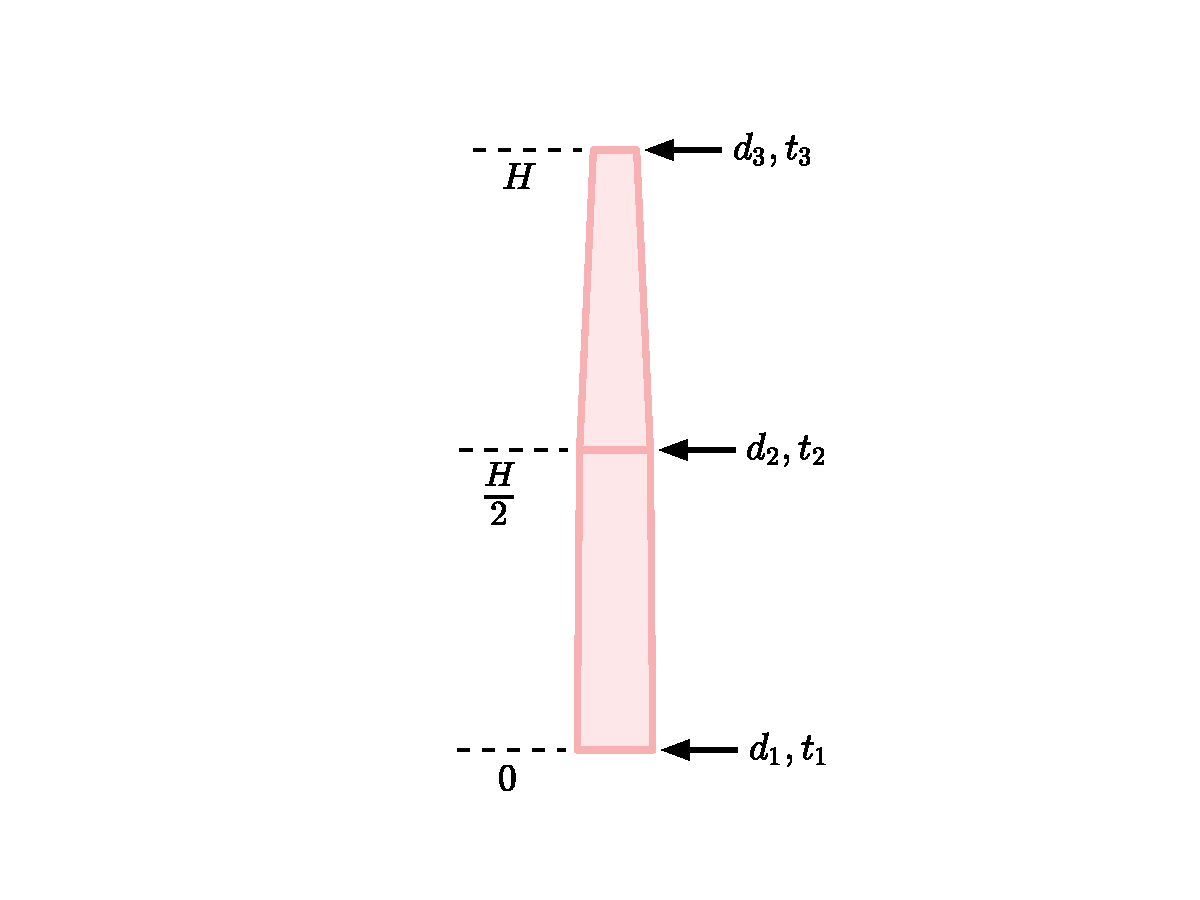
\includegraphics[width=0.5\textwidth]{Figures/tower_param.pdf}
 % \caption{\label{tower_def} The parameterized turbine tower definition. The tower diameter and shell thickness are defined at the bottom, midpoint, and top of the tower, with the values linearly interpolated in between.}
%\end{figure}

\iffalse
The tower mass was a simple calculation from the volume of the tower, the gradients solved by hand.
We calculated shell buckling as a function of the tower geometry and the stresses at each location, following the method outlined in Eurocode \citep{en19931}. These calculations were made in Fortran 90 for speed, and exact gradients were obtained with the Tapenade automatic differentiation tool \citep{hascoet2013tapenade}. We simplified the frequency calculation by approximating the tower as a cantilever beam of constant cross section with an end mass, and used the method described by Erturk et al.\ to calculate the natural frequency \citep{erturk2011appendix}. Because the turbine tower does not in reality 
%Katie: "does not really" sounds casual
have a constant mass density along the length and the mass from the rotor nacelle assembly is slightly offset at the top, our calculation is slightly more conservative than that predicted by TowerSE by about 10\%. 
%Consider instead for flow and clarity: is slightly more conservative than that predicted by TowerSE, about 10\% more conservative 
%more conservative could be replaced by lower frequency or higher frequency depending on what conservative means in this case. 
For this reason we scaled our frequency calculation by 10\% to more closely match the frequency calculated by TowerSE. We chose this simplified model so that we could find gradients, which were obtained using analytic sensitivity equations. 
\fi